% 方向导数

\pentry{全微分\upref{TDiff}, 点乘\upref{Dot}, 正交归一基\upref{OrNrB}}

先来看一幅等高线图(\autoref{DerDir_fig1}). 令高度 $z$ 为位置的函数$z = f(\vec r)$. 这里 $\vec r$ 是位矢\upref{Disp}, 即 $f(\vec r) = f(x,y)$. 当位矢沿着等高线移动时, $z$ 不变,而当位矢沿垂直于等高线的方向移动时, $z$ 变化得最快.位置沿其他方向运动, $z$ 的变化速度介于两者之间.

\begin{figure}[ht]
\centering
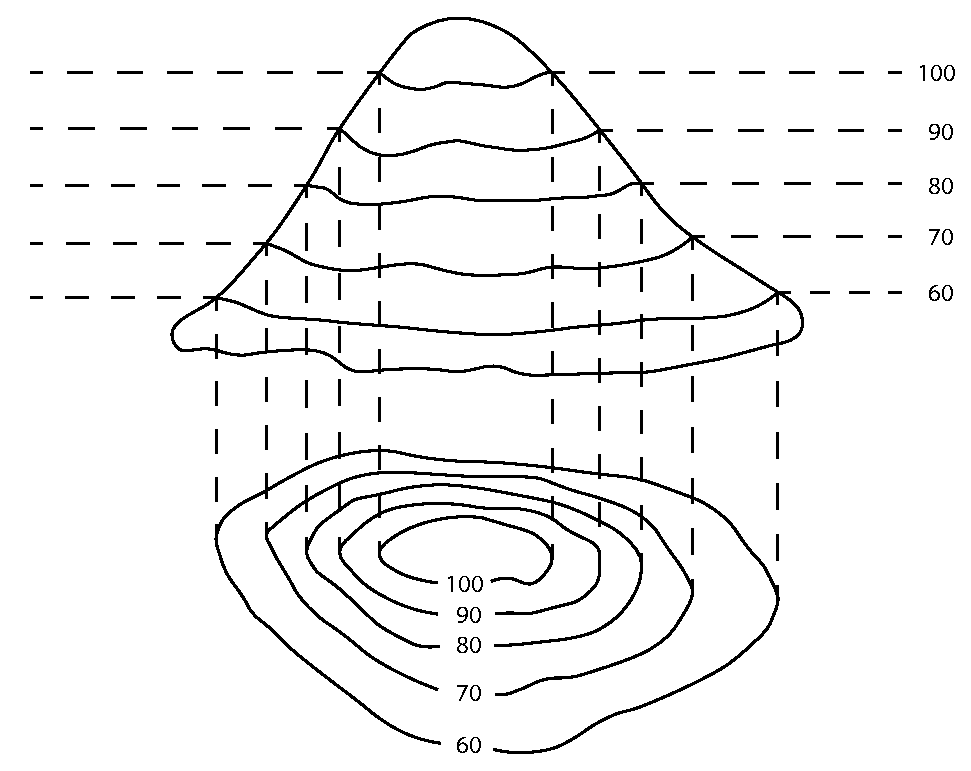
\includegraphics[width=9cm]{./figures/DerDir.pdf}
\caption{等高线}\label{DerDir_fig1}
\end{figure}

那么如何衡量位置向各个方向移动时 $z$ 变化的快慢呢? 我们先规定一个方向 $\uvec n = (n_x,n_y)$( 平面单位矢量,满足 $n_x^2 + n_y^2 = 1$), 然后用\textbf{方向导数}来衡量变化率,其定义如下
 \begin{equation}
\dv{f}{n} \equiv \lim_{\Delta s \to 0} \frac{f(\vec r + \uvec n\Delta s) - f(\vec r)}{\Delta s} = \dv{f}{s}
\end{equation}
其中 $\uvec n\Delta s$ 代表沿 $\uvec n$ 方向的微小位移.从几何上来讲,二维函数 $f(\vec r)$ 表示一个曲面,曲面上某点的方向导数就是曲面在该方向的斜率.


% 以下的解释应该给全微分! 这里直接引用全微分的结论即可!
由“全微分\upref{TDiff}”中的结论
\begin{equation}
\dd{f} = \pdv{f}{x} \dd{x} + \pdv{f}{y} \dd{y}
\end{equation}
而现在我们往 $\uvec n = (n_x, n_y)$ 方向移动 $\dd{s}$,所以
\begin{equation}
\dd{x} = n_x \dd{s} \qquad \dd{y} = n_y \dd{s}
\end{equation}
代入上式,得
\begin{equation}
\dd{f} =  \qty(\pdv{f}{x} n_x + \pdv{f}{y} n_y ) \dd{s}
\end{equation}
根据导数与微分的关系(也可以通俗地说“两边同除 $\dd{s}$”), 就得到方向导数
\begin{equation}
\pdv{f}{n} = \dv{f}{s} = \pdv{f}{x} n_x + \pdv{f}{y} n_y
\end{equation}
如果使用平面的正交归一基\upref{OrNrB} $\uvec x, \uvec y$ 写成矢量点乘\upref{Dot} 的形式,就是
\begin{equation}
\dv{f}{n} = \qty( \pdv{f}{x}\uvec x + \pdv{f}{y}\uvec y ) \vdot \uvec n
\end{equation} 
定义\textbf{二维直角坐标系中的 Del 算符}为
\begin{equation}
\grad  = \uvec x\pdv{x} + \uvec y\pdv{y}
\end{equation}
其作用在函数上表示
\begin{equation}
\grad f = \pdv{f}{x}\uvec x + \pdv{f}{y}\uvec y
\end{equation} 
则方向导数可以写成相当简洁的形式,即
\begin{equation}\label{DerDir_eq7}
\pdv{f}{n} = \grad f \vdot \uvec n
\end{equation} 

\subsection{多元函数的方向导数}
通过和以上类似的分析,可以得出 $N$ 元函数 $f(\vec r) = f(x_1,x_2\dots x_N)$ 在单位方向矢量 $\uvec n = (n_{x1}, n_{x2} \dots n_{x_N})$ 的方向上的微分关系为
\begin{equation}
\dd{f} = \pdv{f}{x_1} \dd{x_1} + \pdv{f}{x_2} \dd{x_2}\ldots = \qty( \pdv{f}{x_1}n_{x1} + \pdv{f}{x_2} n_{x2}\dots ) \dd{s}
\end{equation}
方向导数为
\begin{equation}
\pdv{f}{n} = \dv{f}{s} = \qty( \pdv{f}{x_1}\uvec x_1 + \pdv{f}{x_2}\uvec x_2\ldots  \pdv{f}{x_N}\uvec x_N ) \vdot \uvec n = \grad f \vdot \uvec n
\end{equation} 
形式与\autoref{DerDir_eq7} 相同.这里定义了\textbf{ $N$ 维直角坐标系的 Del 算符} 为
\begin{equation}
\grad  = \uvec x_1\pdv{f}{x_1} + \uvec x_2\pdv{f}{x_2} \dots \uvec x_n\pdv{f}{x_N}
\end{equation}


